\documentclass[]{article}
\usepackage[left=1in,top=1in,right=1in,bottom=1in]{geometry}


%%%% more monte %%%%
% thispagestyle{empty}
% https://stackoverflow.com/questions/2166557/how-to-hide-the-page-number-in-latex-on-first-page-of-a-chapter
\usepackage{color}
% \usepackage[table]{xcolor} % are they using color?

% \definecolor{WSU.crimson}{HTML}{981e32}
% \definecolor{WSU.gray}{HTML}{5e6a71}

% \definecolor{shadecolor}{RGB}{248,248,248}
\definecolor{WSU.crimson}{RGB}{152,30,50} % use http://colors.mshaffer.com to convert from 981e32
\definecolor{WSU.gray}{RGB}{94,106,113}

%%%%%%%%%%%%%%%%%%%%%%%%%%%%

\newcommand*{\authorfont}{\fontfamily{phv}\selectfont}
\usepackage{lmodern}


  \usepackage[T1]{fontenc}
  \usepackage[utf8]{inputenc}




\usepackage{abstract}
\renewcommand{\abstractname}{}    % clear the title
\renewcommand{\absnamepos}{empty} % originally center

\renewenvironment{abstract}
 {{%
    \setlength{\leftmargin}{0mm}
    \setlength{\rightmargin}{\leftmargin}%
  }%
  \relax}
 {\endlist}

\makeatletter
\def\@maketitle{%
  \pagestyle{empty}
  \newpage
%  \null
%  \vskip 2em%
%  \begin{center}%
  \let \footnote \thanks
    {\fontsize{18}{20}\selectfont\raggedright  \setlength{\parindent}{0pt} \@title \par}%
}
%\fi
\makeatother






\usepackage{color}
\usepackage{fancyvrb}
\newcommand{\VerbBar}{|}
\newcommand{\VERB}{\Verb[commandchars=\\\{\}]}
\DefineVerbatimEnvironment{Highlighting}{Verbatim}{commandchars=\\\{\}}
% Add ',fontsize=\small' for more characters per line
\usepackage{framed}
\definecolor{shadecolor}{RGB}{248,248,248}
\newenvironment{Shaded}{\begin{snugshade}}{\end{snugshade}}
\newcommand{\AlertTok}[1]{\textcolor[rgb]{0.94,0.16,0.16}{#1}}
\newcommand{\AnnotationTok}[1]{\textcolor[rgb]{0.56,0.35,0.01}{\textbf{\textit{#1}}}}
\newcommand{\AttributeTok}[1]{\textcolor[rgb]{0.77,0.63,0.00}{#1}}
\newcommand{\BaseNTok}[1]{\textcolor[rgb]{0.00,0.00,0.81}{#1}}
\newcommand{\BuiltInTok}[1]{#1}
\newcommand{\CharTok}[1]{\textcolor[rgb]{0.31,0.60,0.02}{#1}}
\newcommand{\CommentTok}[1]{\textcolor[rgb]{0.56,0.35,0.01}{\textit{#1}}}
\newcommand{\CommentVarTok}[1]{\textcolor[rgb]{0.56,0.35,0.01}{\textbf{\textit{#1}}}}
\newcommand{\ConstantTok}[1]{\textcolor[rgb]{0.00,0.00,0.00}{#1}}
\newcommand{\ControlFlowTok}[1]{\textcolor[rgb]{0.13,0.29,0.53}{\textbf{#1}}}
\newcommand{\DataTypeTok}[1]{\textcolor[rgb]{0.13,0.29,0.53}{#1}}
\newcommand{\DecValTok}[1]{\textcolor[rgb]{0.00,0.00,0.81}{#1}}
\newcommand{\DocumentationTok}[1]{\textcolor[rgb]{0.56,0.35,0.01}{\textbf{\textit{#1}}}}
\newcommand{\ErrorTok}[1]{\textcolor[rgb]{0.64,0.00,0.00}{\textbf{#1}}}
\newcommand{\ExtensionTok}[1]{#1}
\newcommand{\FloatTok}[1]{\textcolor[rgb]{0.00,0.00,0.81}{#1}}
\newcommand{\FunctionTok}[1]{\textcolor[rgb]{0.00,0.00,0.00}{#1}}
\newcommand{\ImportTok}[1]{#1}
\newcommand{\InformationTok}[1]{\textcolor[rgb]{0.56,0.35,0.01}{\textbf{\textit{#1}}}}
\newcommand{\KeywordTok}[1]{\textcolor[rgb]{0.13,0.29,0.53}{\textbf{#1}}}
\newcommand{\NormalTok}[1]{#1}
\newcommand{\OperatorTok}[1]{\textcolor[rgb]{0.81,0.36,0.00}{\textbf{#1}}}
\newcommand{\OtherTok}[1]{\textcolor[rgb]{0.56,0.35,0.01}{#1}}
\newcommand{\PreprocessorTok}[1]{\textcolor[rgb]{0.56,0.35,0.01}{\textit{#1}}}
\newcommand{\RegionMarkerTok}[1]{#1}
\newcommand{\SpecialCharTok}[1]{\textcolor[rgb]{0.00,0.00,0.00}{#1}}
\newcommand{\SpecialStringTok}[1]{\textcolor[rgb]{0.31,0.60,0.02}{#1}}
\newcommand{\StringTok}[1]{\textcolor[rgb]{0.31,0.60,0.02}{#1}}
\newcommand{\VariableTok}[1]{\textcolor[rgb]{0.00,0.00,0.00}{#1}}
\newcommand{\VerbatimStringTok}[1]{\textcolor[rgb]{0.31,0.60,0.02}{#1}}
\newcommand{\WarningTok}[1]{\textcolor[rgb]{0.56,0.35,0.01}{\textbf{\textit{#1}}}}



\title{\textbf{\textcolor{WSU.crimson}{How Age Affects Physical
Attributes}} \newline \textbf{\textcolor{WSU.gray}{Exploring An Answered
Question}}  }
 

%  

% \author{ \Large true \hfill \normalsize \emph{} }
\author{\Large Christopher
Sarno\vspace{0.05in} \newline\normalsize\emph{Washington State
University}  }


\date{December 11, 2020}
\setcounter{secnumdepth}{3}

\usepackage{titlesec}
% See the link above: KOMA classes are not compatible with titlesec any more. Sorry.
% https://github.com/jbezos/titlesec/issues/11
\titleformat*{\section}{\bfseries}
\titleformat*{\subsection}{\bfseries\itshape}
\titleformat*{\subsubsection}{\itshape}
\titleformat*{\paragraph}{\itshape}
\titleformat*{\subparagraph}{\itshape}

% https://code.usgs.gov/usgs/norock/irvine_k/ip-092225/


%\titleformat*{\section}{\normalsize\bfseries}
%\titleformat*{\subsection}{\normalsize\itshape}
%\titleformat*{\subsubsection}{\normalsize\itshape}
%\titleformat*{\paragraph}{\normalsize\itshape}
%\titleformat*{\subparagraph}{\normalsize\itshape}

% https://tex.stackexchange.com/questions/233866/one-column-multicol-environment#233904
\usepackage{environ}
\NewEnviron{auxmulticols}[1]{%
  \ifnum#1<2\relax% Fewer than 2 columns
    %\vspace{-\baselineskip}% Possible vertical correction
    \BODY
  \else% More than 1 column
    \begin{multicols}{#1}
      \BODY
    \end{multicols}%
  \fi
}





\usepackage{natbib}
\setcitestyle{aysep={}} %% no year, comma just year
% \usepackage[numbers]{natbib}
\bibliographystyle{./biblio/ormsv080.bst}



\usepackage[strings]{underscore} % protect underscores in most circumstances




\newtheorem{hypothesis}{Hypothesis}
\usepackage{setspace}


%%%%%%%%%%%%%%%%%%%%%%%%%%%%%%%%%%%%%%%%%%%%%%%%%%%%%
%%% MONTE ADDS %%%

\usepackage{fancyhdr} % fancy header 
\usepackage{lastpage} % last page 

\usepackage{multicol}


\usepackage{etoolbox}
\AtBeginEnvironment{quote}{\singlespacing\small}
% https://tex.stackexchange.com/questions/325695/how-to-style-blockquote


\usepackage{soul}			%% allows strike-through
\usepackage{url}			%% fixes underscores in urls
\usepackage{csquotes}		%% allows \textquote in references
\usepackage{rotating}		%% allows table and box rotation
\usepackage{caption}		%% customize caption information
\usepackage{booktabs}		%% enhance table/tabular environment
\usepackage{tabularx}		%% width attributes updates tabular
\usepackage{enumerate}		%% special item environment
\usepackage{enumitem}		%% special item environment

\usepackage{lineno}		%% allows linenumbers for editing using \linenumbers
\usepackage{hanging}


\usepackage{mathtools}  	%% also loads amsmath
\usepackage{bm}		%% bold-math
\usepackage{scalerel}	%% scale one element (make one beta bigger font)

\newcommand{\gFrac}[2]{ \genfrac{}{}{0pt}{1}{{#1}}{#2} }

\newcommand{\betaSH}[3]{  \gFrac{\text{\tiny #1}}{{\text{\tiny #2}}}\hat{\beta}_{\text{#3}}   }
\newcommand{\betaSB}[3]{              ^{\text{#1}} _{\text{#2}} \bm{\beta} _{\text{#3}}                   }  %% bold
\newcommand{\bigEQ}{  \scaleobj{1.5}{{\ }= } }
\newcommand{\bigP}[1]{  \scaleobj{1.5}{#1 } }





\usepackage{endnotes}  % he already does this ...
\renewcommand{\enotesize}{\normalsize}
% https://tex.stackexchange.com/questions/99984/endnotes-do-not-be-superscript-and-add-a-space
\renewcommand\makeenmark{\textsuperscript{[\theenmark]}} % in brackets %
% https://tex.stackexchange.com/questions/31574/how-to-control-the-indent-in-endnotes
\patchcmd{\enoteformat}{1.8em}{0pt}{}{}

\patchcmd{\theendnotes}
  {\makeatletter}
  {\makeatletter\renewcommand\makeenmark{\textbf{[\theenmark]} }}
  {}{}



% https://tex.stackexchange.com/questions/141906/configuring-footnote-position-and-spacing

\addtolength{\footnotesep}{5mm} % change to 1mm

\renewcommand{\thefootnote}{\textbf{\arabic{footnote}}}
\let\footnote=\endnote
%\renewcommand*{\theendnote}{\alph{endnote}}
%\renewcommand{\theendnote}{\textbf{\arabic{endnote}}}


\renewcommand*{\notesname}{ENDNOTES}

\makeatletter
\def\enoteheading{\section*{\notesname
  \@mkboth{\MakeUppercase{\notesname}}{\MakeUppercase{\notesname}}}%
  \mbox{}\par\vskip-2.3\baselineskip\noindent\rule{.5\textwidth}{0.4pt}\par\vskip\baselineskip}
\makeatother


\renewcommand*{\contentsname}{TABLE OF CONTENTS}

\renewcommand*{\refname}{REFERENCES}


%\usepackage{subfigure}
\usepackage{subcaption}

\captionsetup{labelfont=bf}  % Make Table / Figure bold

%%% you could add elements here ... monte says .... %%%
%\usepackage{mypackageForCapitalH}


%%%%%%%%%%%%%%%%%%%%%%%%%%%%%%%%%%%%%%%%%%%%%%%%%%%%%

% set default figure placement to htbp
\makeatletter
\def\fps@figure{htbp}
\makeatother


% move the hyperref stuff down here, after header-includes, to allow for - \usepackage{hyperref}

\makeatletter
\@ifpackageloaded{hyperref}{}{%
\ifxetex
  \PassOptionsToPackage{hyphens}{url}\usepackage[setpagesize=false, % page size defined by xetex
              unicode=false, % unicode breaks when used with xetex
              xetex]{hyperref}
\else
  \PassOptionsToPackage{hyphens}{url}\usepackage[draft,unicode=true]{hyperref}
\fi
}

\@ifpackageloaded{color}{
    \PassOptionsToPackage{usenames,dvipsnames}{color}
}{%
    \usepackage[usenames,dvipsnames]{color}
}
\makeatother
\hypersetup{breaklinks=true,
            bookmarks=true,
            pdfauthor={Christopher Sarno (Washington State University)},
             pdfkeywords = {multiple comparisons to control; correlation
strength; nonlinear growth curves; critical points},  
            pdftitle={How Age Affects Physical Attributes: Exploring An
Answered Question},
            colorlinks=true,
            citecolor=blue,
            urlcolor=blue,
            linkcolor=magenta,
            pdfborder={0 0 0}}
\urlstyle{same}  % don't use monospace font for urls

% Add an option for endnotes. -----

%
% add tightlist ----------
\providecommand{\tightlist}{%
\setlength{\itemsep}{0pt}\setlength{\parskip}{0pt}}

% add some other packages ----------

% \usepackage{multicol}
% This should regulate where figures float
% See: https://tex.stackexchange.com/questions/2275/keeping-tables-figures-close-to-where-they-are-mentioned
\usepackage[section]{placeins}



\pagestyle{fancy}   
\lhead{\textcolor{WSU.crimson}{\textbf{ How Age Affects Physical
Attributes }}}
\chead{}
\rhead{\textcolor{WSU.gray}{\textbf{  Page\ \thepage\ of\ \protect\pageref{LastPage} }}}
\lfoot{}
\cfoot{}
\rfoot{}


\begin{document}
	
% \pagenumbering{arabic}% resets `page` counter to 1 
%    

% \maketitle

{% \usefont{T1}{pnc}{m}{n}
\setlength{\parindent}{0pt}
\thispagestyle{plain}
{\fontsize{18}{20}\selectfont\raggedright 
\maketitle  % title \par  

}

{
   \vskip 13.5pt\relax \normalsize\fontsize{11}{12} 
   
\textbf{\authorfont Christopher
Sarno} \hskip 15pt \emph{\small Washington State University}   

}

}








\begin{abstract}

    \hbox{\vrule height .2pt width 39.14pc}

    \vskip 8.5pt % \small 

\noindent In this article we compare how \emph{age} correlates to and
affects a variety of variables, including \emph{height},
\emph{floor to hip length}, and \emph{hip to head length}. The goal is
to reject or fail to reject a null hypothesis that age affects these
physical attributes equally. \vspace{0.25in}


\vskip 8.5pt \noindent \textbf{\underline{Keywords}:} multiple
comparisons to control; correlation strength; nonlinear growth curves;
critical points \par

    




    
    \hbox{\vrule height .2pt width 39.14pc}
    \vskip 5pt 
    \hfill \textbf{\textcolor{WSU.gray}{ December 11, 2020 } }
    \vskip 5pt 
    
\end{abstract}


\vskip -8.5pt



 % removetitleabstract

\noindent  

\section{Introduction}
\label{sec:intro}

Age affects everyone differently. The question that stood out to me when
looking at the measure data was how age correlates with height, whether
different parts of the body grew quicker than others, and if gender was
a factor.

I decided to narrow down the comparisons to the few attributes listed
above for their close relation to each other. Hip to floor is the height
of the lower half of the body and we can find the height of the upper
half of the body by subtracting the height of the lower half from the
full height. This measurement is later referred to as ``hip to head''.

\begin{figure}[!ht]
%% figures have hrule, tables have hline
    \hrule
    \caption{ \textbf{Conceptual Model} }
    \begin{center}
        \scalebox{1.00}{    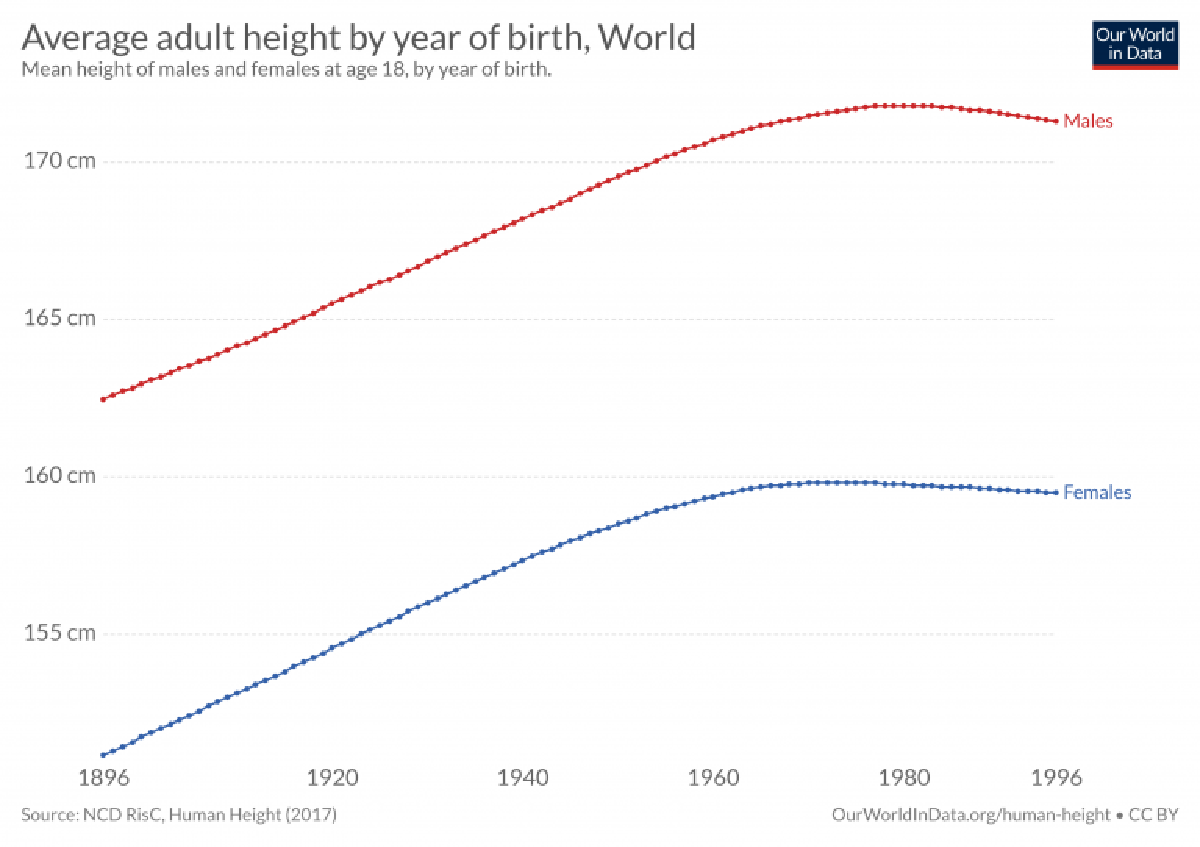
\includegraphics[trim = 0 0 0 0,clip,width=\textwidth]{figures/heightbyyear.pdf} }
    \end{center}
    \label{fig:conceptual-model}
  \hrule
  \vspace{2.5mm}
      \caption{\textbf{ A look at average adult height throughout the past century }   }
      \label{fig:combined}
  \vspace{-2.5mm}
  \hrule
\end{figure}
\newpage

\begin{figure}[!ht]
%% figures have hrule, tables have hline
    \hrule
    \caption{ \textbf{Conceptual Model} }
    \begin{center}
        \scalebox{1.00}{    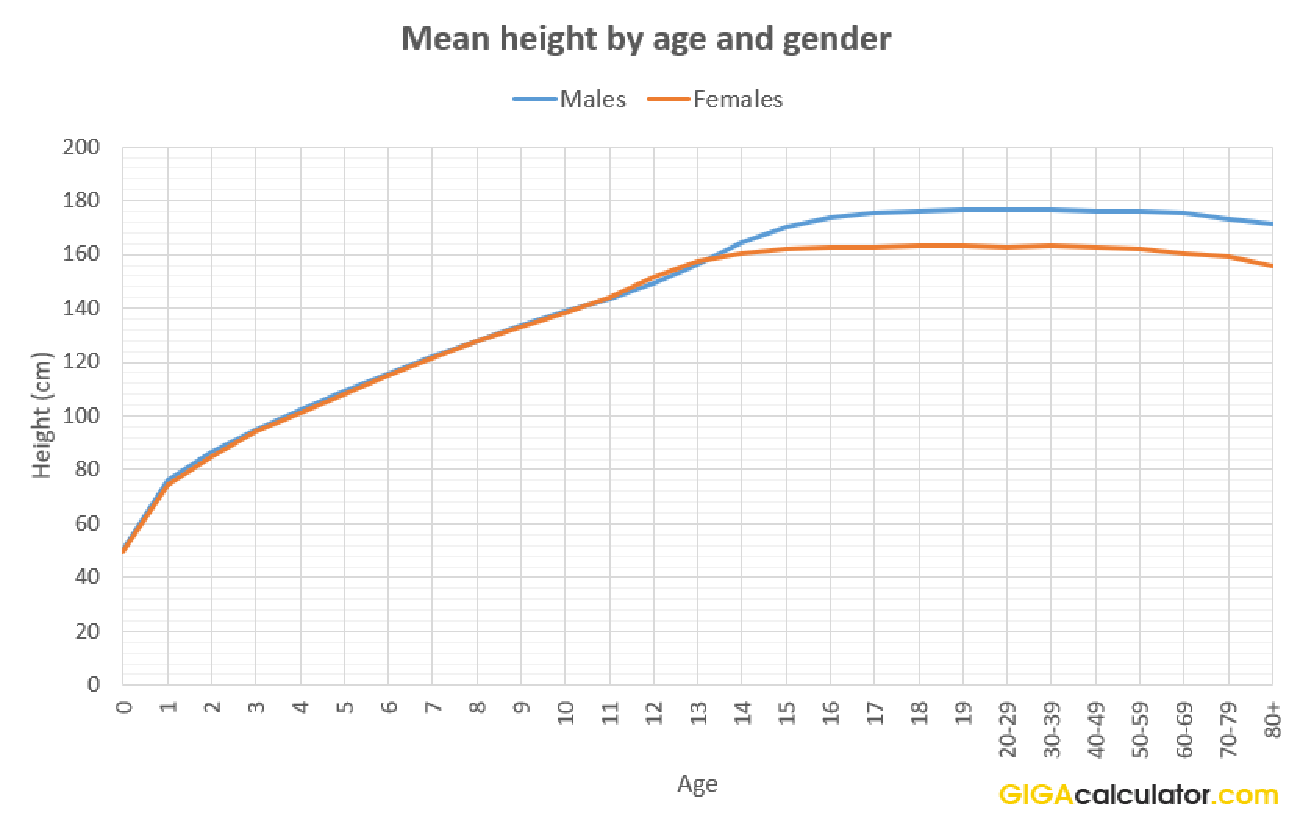
\includegraphics[trim = 0 0 0 0,clip,width=\textwidth]{figures/conceptualgraph2.pdf} }
    \end{center}
    \label{fig:conceptual-mean}
    \hrule
\end{figure}
\newpage

See Figure \ref{fig:conceptual-mean}.

\section{Research Question:  The primary research question for this article is as follows: What is the age people start and stop growing? }
\label{sec:rq}

\subsection{Secondary question: Do different attributes scale differently with age than others? }
\label{sec:rq2}

\subsection{Tertiary question: How strong is the correlation between age and height, and between those different attributes?}
\label{sec:rq3}

\newpage

\section{Data Description}
\label{sec:data}

The circumstances surrounding the gathering of this data was quite
abnormal. Due to the Covid-19 pandemic, in-person data collection was
just about off the table. A data collection sheet was instead drafted
up, asking the participants to enter a number of personal information
including covariates such as age, ethnicity, and gender, and a plethora
of physical measurements.

The data collection handout was distributed virtually to ten
participants per analyst and the data was compiled into one large
database. Names of the participants were run through a md5 text
converted, assuring anonymity.

\subsection{Summary of Sample}
\label{sec:data-sample}

\begin{figure}[!ht]
%% figures have hrule, tables have hline
    \hrule
    \caption{ \textbf{Summary Of Data} }
    \begin{center}
        \scalebox{1.00}{    \includegraphics[trim = 0 0 0 0,clip,width=\textwidth]{figures/summary.pdf} }
    \end{center}
    \label{fig:summary}
    \hrule
\end{figure}
\newpage

\subsection{Summary Statistics of Data}
\label{sec:data-summary}

\begin{figure}[!ht]
%% figures have hrule, tables have hline
    \hrule
    \caption{ \textbf{Conceptual Model} }
    \begin{center}
        \scalebox{1.00}{    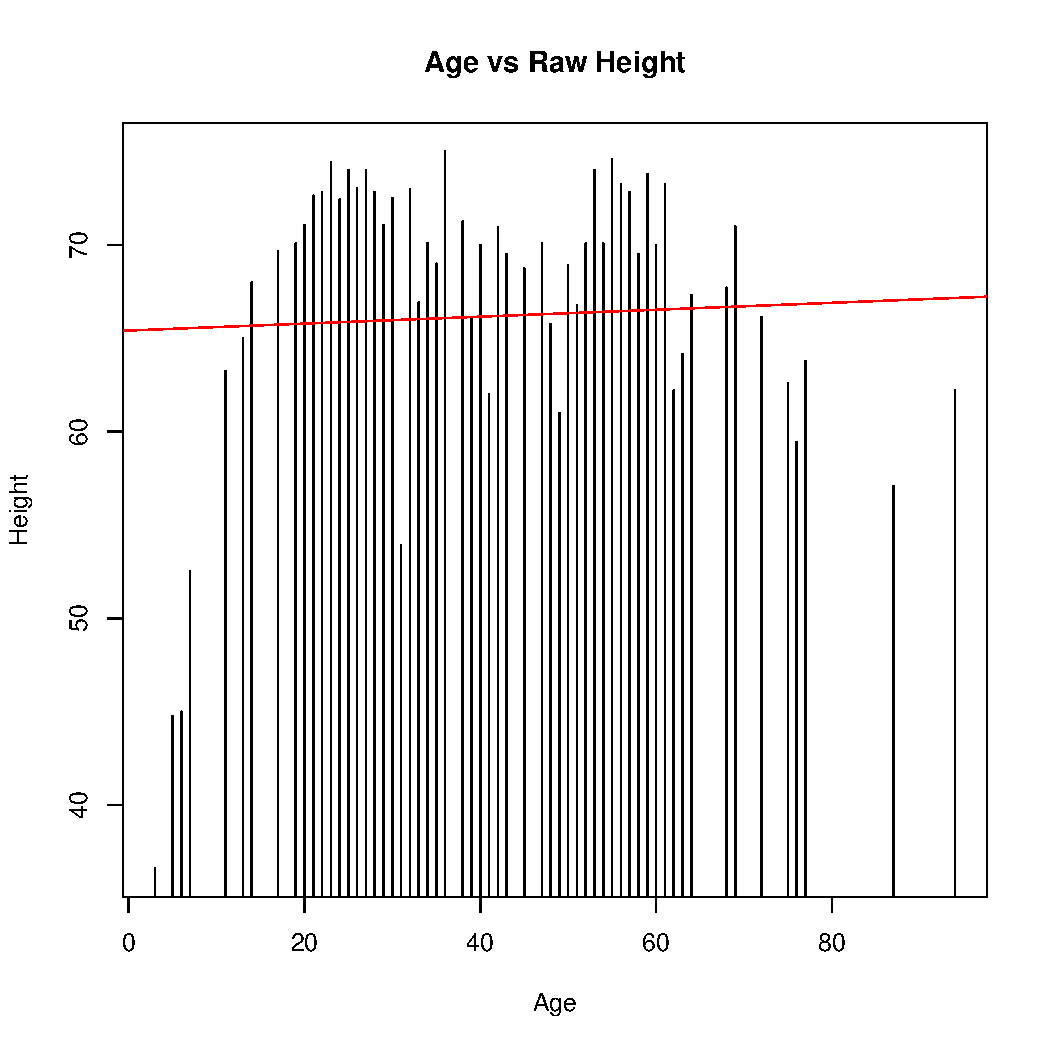
\includegraphics[trim = 0 0 0 0,clip,width=\textwidth]{figures/height-graph.pdf} }
    \end{center}
    \label{fig:age-height-graph}
  \hrule
  \vspace{2.5mm}
      \caption{\textbf{ A histogram-like age vs height plot }   }
      \label{fig:combined}
  \vspace{-2.5mm}
  \hrule
\end{figure}

\begin{figure}[!ht]
%% figures have hrule, tables have hline
    \hrule
    \caption{ \textbf{Lower Half} }
    \begin{center}
        \scalebox{1.00}{    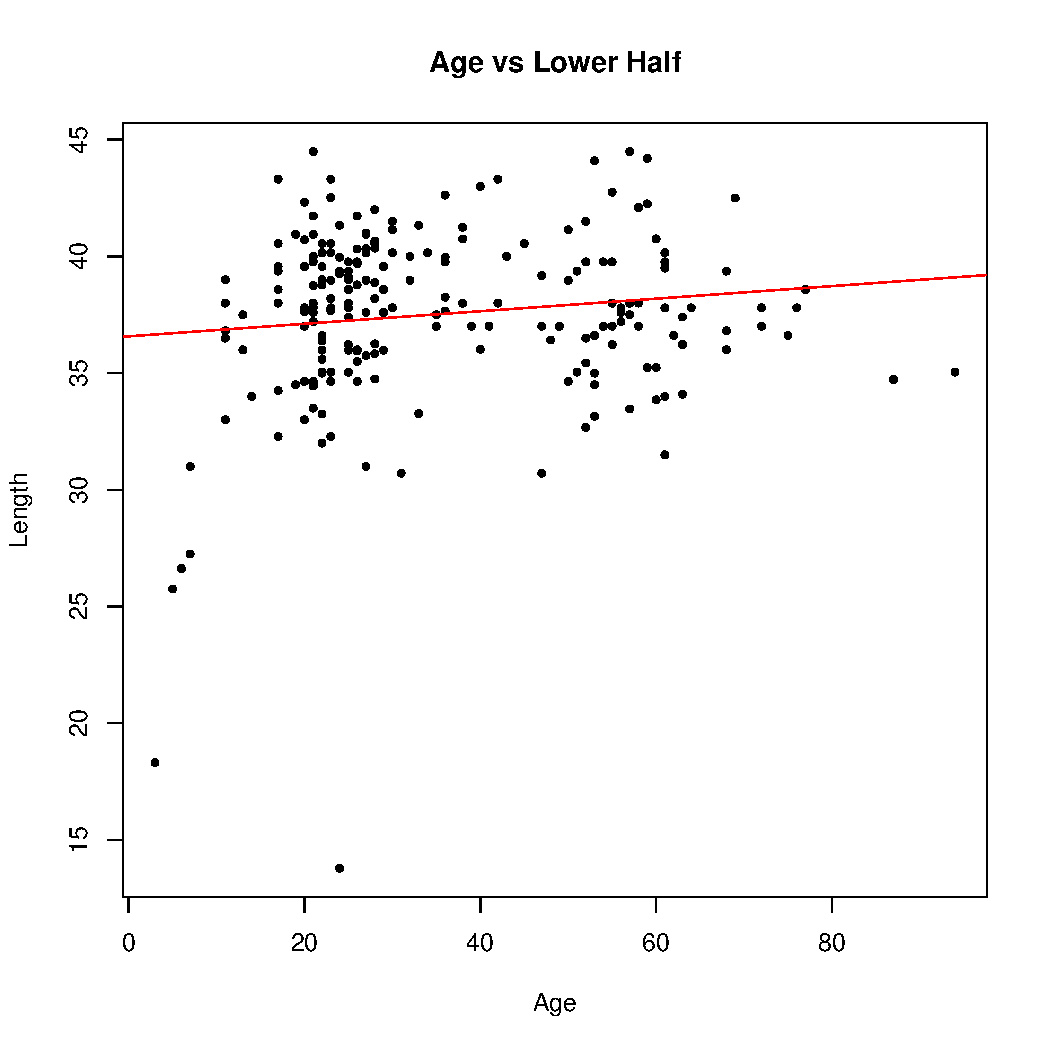
\includegraphics[trim = 0 0 0 0,clip,width=\textwidth]{figures/hip-floor-graph.pdf} }
    \end{center}
    \label{fig:hip-floor-graph}
  \hrule
  \vspace{2.5mm}
      \caption{\textbf{ Plotting Age Vs Hip To Floor Measurement }   }
      \label{fig:combined}
  \vspace{-2.5mm}
  \hrule
\end{figure}
\newpage

\begin{figure}[!ht]
%% figures have hrule, tables have hline
    \hrule
    \caption{ \textbf{Upper Half} }
    \begin{center}
        \scalebox{1.00}{    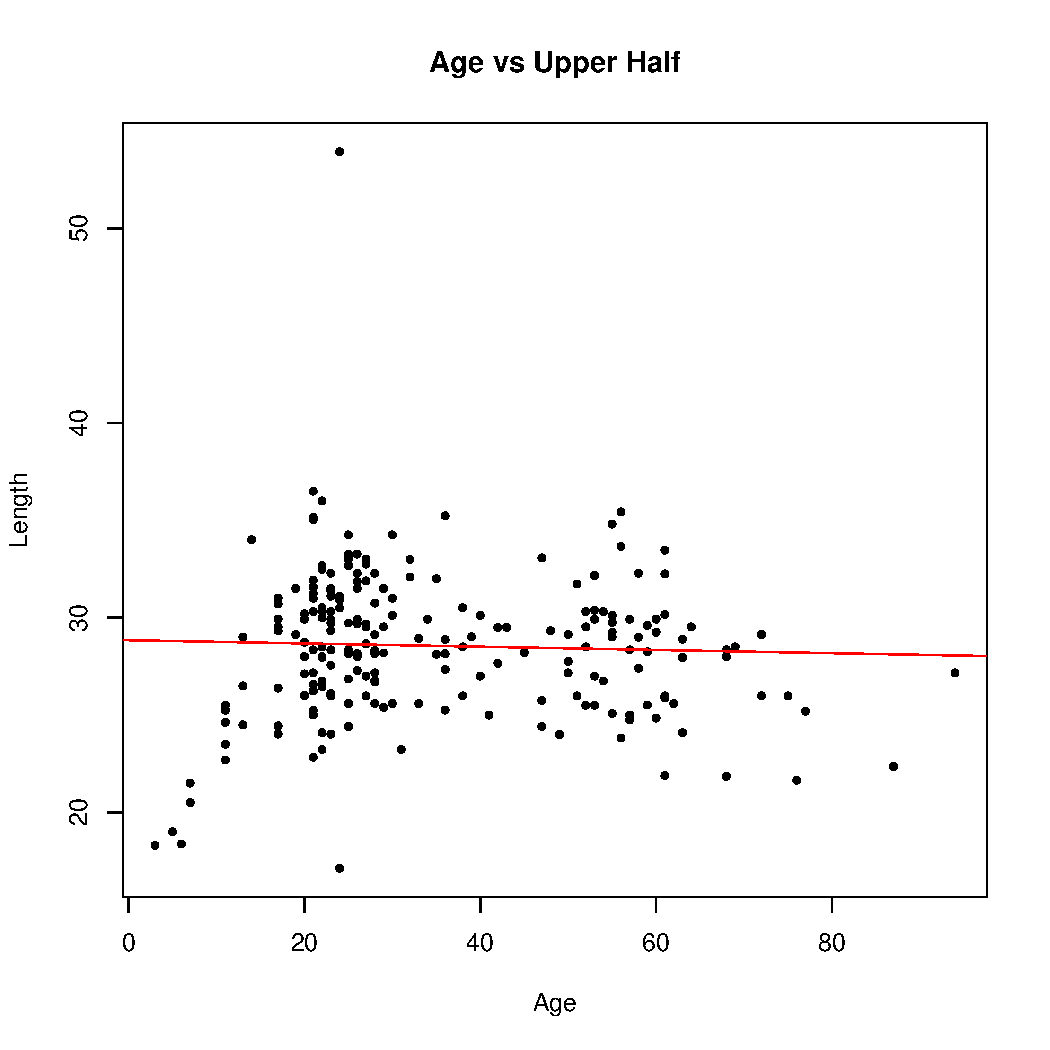
\includegraphics[trim = 0 0 0 0,clip,width=\textwidth]{figures/hip-head-graph.pdf} }
    \end{center}
    \label{fig:hip-head-graph}
  \hrule
  \vspace{2.5mm}
      \caption{\textbf{ Plotting Age Vs Hip To Head Measurement }   }
      \label{fig:combined}
  \vspace{-2.5mm}
  \hrule
\end{figure}
\newpage

\section{Key Findings}
\label{sec:findings}

Beginning with the primary research question, Figure
\ref{fig:age-height-graph} indicates that growth begins very rapidly
almost immediately after birth, and begins to plateau soon after age 20.
Interestingly, the few datapoints we have for the height of those over
the age of 60 indicates that height seems to regress a bit after age 60.
However, due to the extremes at both ends, the correlation between age
and height is very weak at 0.06.

To answer the secondary and tertiary questions regarding how different
physical attributes scale with height, if they scale independently of
one another, and their correlations, we will refer to the scatterplots,
their regression lines, and correlation values. Figure
\ref{fig:hip-floor-graph} shows a constant, positive trend between age
and the length from hip to floor. The scatterplot loosely follows that
of the height graph, but with a bit more variation. However, the
correlation between age and lower half height is quite weak with a value
of only 0.128. While this is

We can compare this to Figure \ref{fig:hip-head-graph}, which shows a
constant, slightly negative trend between age and the length from hip to
head. Again, however, the correlation between age and the length from
hip to head is extremely weak and surprisingly negative at -0.04,
indicating that the length between a person's hip and their head
decreases with age.

While all referenced correlations are weak, it is significant to point
out the difference between the rate at which age scales with the lengths
of the upper half and lower half of the body. Ignoring intercepts, the
length from floor to hip scales positively with 0.0269 times age yet the
length from hip to head scales negatively with -0.008323 times age. This
is a 3.5\% difference in age scaling between the upper half and lower
half of the body, which is not an insignificant amount.

\section{Conclusion}
\label{sec:conclusion}

To summarize the answers to our research questions, the critical points
for growth are located at birth (x=0) and around age 20. Growth begins
immediately and very rapidly starting at the first critical point, then
tapers off and stagnates at the second critical point. While the
scatterplots show that the upper half and the lower half of the body
scale inversely and independently with age, the correlation between the
three factors is too low to make a statement with any real confidence.
Therefore, we fail to reject the null hypothesis that age affects the
selected physical attributes equally. \newpage

\vspace{0.5in}

\newpage

Refer to the Appendices in section\textasciitilde{}\ref{sec:appendix}
where I am going to cite John \citep[pp. 2-3]{Tukey:1962}.

Here is a quote by \citet[pp. 2-3]{Tukey:1962}:

\begin{quote}
For a long time I have thought I was a statistician, interested in inferences from the particular to the general.  But as I have watched mathematical statistics evolve, I have had to cause to wonder and to doubt. [...] All in all, I have come to feel that my central interest is in \emph{data analysis}, which I take to include among other things: procedures for analyzing data, techniques for interpreting the results of such procedures, ways of planning the gathering of data to make its analysis easier, more precise or more accurate, and all the machinery and results of (mathematical) statistics which apply to analyzing the data.

Large parts of data analysis are inferential in the sample-to-population sense, but these are only parts, not the whole.  Large parts of data analysis are incisive, laying bare indications which we could not perceive by simple and direct examination of the raw data, but these too are only parts, not the whole.  Some parts of data analysis, as the term is her stretch beyond its philology, are allocation, in the sense that they guide us in the distribution of effort and other valuable considerations in observation, experimentation, or analysis.  Data analysis is a larger and more varied field than inference, or incisive procedures, or allocation.

Statistics has contributed much to data analysis.  In the future it can, and in my view should, contribute more.  For such contributions to exist, and be valuable, it is not necessary that they be direct.  They need not provide new techniques, or better tables for old techniques, in order to influence the practice of data analysis.
\end{quote}

\newpage

\begin{table}[!htbp]
\footnotesize
\centering
\caption{\textbf{Descriptive Statistics and Correlation Analysis}}
\label{table:correlation}
\begin{tabularx}{0.75\textwidth}{{r@{ \ \ } p{35mm} r@{}lp{1mm} r@{}l p{5mm} r@{}l p{2mm} r@{}l p{2mm} r@{}l p{2mm}   r@{}l  }}
 & \\
\hline
 & \\
\multicolumn{2}{c}{\textbf{ }} & \multicolumn{2}{c}{\textbf{M}} & & \multicolumn{2}{c}{\textbf{SD}} &  & \multicolumn{2}{c}{\textbf{1}} &  & \multicolumn{2}{c}{\textbf{2}} &  & \multicolumn{2}{c}{\textbf{3}} &  & \\ 
 & \\
\hline
 & \\
\textbf{1} & \textbf{age} &  34&.9 &  &  17&.83 &  &  1&  &  &  \multicolumn{2}{c}{ \  \  \  \  \ }  &  &  \multicolumn{2}{c}{ \  \  \  \  \ }  &  & \\ 
 & \\
\textbf{2} & \textbf{height} &  66&.1 &  &  5&.38 &  &  &.06 &  &  1&  &  &  \multicolumn{2}{c}{ \  \  \  \  \ }  &  & \\ 
 & \\
\textbf{3} & \textbf{floor.hip} &  37&.5 &  &  3&.74 &  &  &.13{$^{\dagger}$}  &  &  &.71{$^{***}$}  &  &  1&  &  & \\ 
 & \\
\textbf{4} & \textbf{NA} &  28&.6 &  &  3&.82 &  &  -&.04 &  &  &.72{$^{***}$}  &  &  &.01 &  & \\ 
 & \\
\hline
 & \\
\multicolumn{16}{p{0.68\textwidth}}{  \footnotesize { \begin{hangparas}{0.75in}{1} \textbf{\underline{Notes}:} \ \ Pearson pairwise correlations are reported; \newline a two-side test was performed to report correlation significance.  \end{hangparas} } }  & \\  
\multicolumn{16}{p{0.68\textwidth}}{  {\tiny {$^{\dagger} p < .10$} }  {     } {\tiny        {$^{*} p < .05$} }  {     } {\tiny       {$^{**} p < .01$} }  {     } {\tiny      {$^{***} p < .001$} } {     }     } & \\ 
 & \\
\hline
\end{tabularx}
\end{table}


\newpage

\newpage
\section{APPENDICES}
\label{sec:appendix}

\subsection{Data Provenance}
\label{sec:appendix-data-provenance}

As stated above, gathering the data from the source was difficult due to
complications from the global pandemic. Since in-person data collection
was impossible, it was impossible to assure impeccable quality of data.

Quality scores for the data was estimated by the analysts but we cannot
be sure of its accuracy. As such, further studies and testing could be
performed only on data that meet certain quality requirements, which
perhaps could influence our analysis and findings presented in this
article.

\newpage
\subsubsection{Data Collection Handout}
\label{sec:appendix-data-handout}

\begin{figure}[!ht]
    \hrule
    \caption{ \textbf{Handout} }
    \begin{center}
        \scalebox{1.00}{    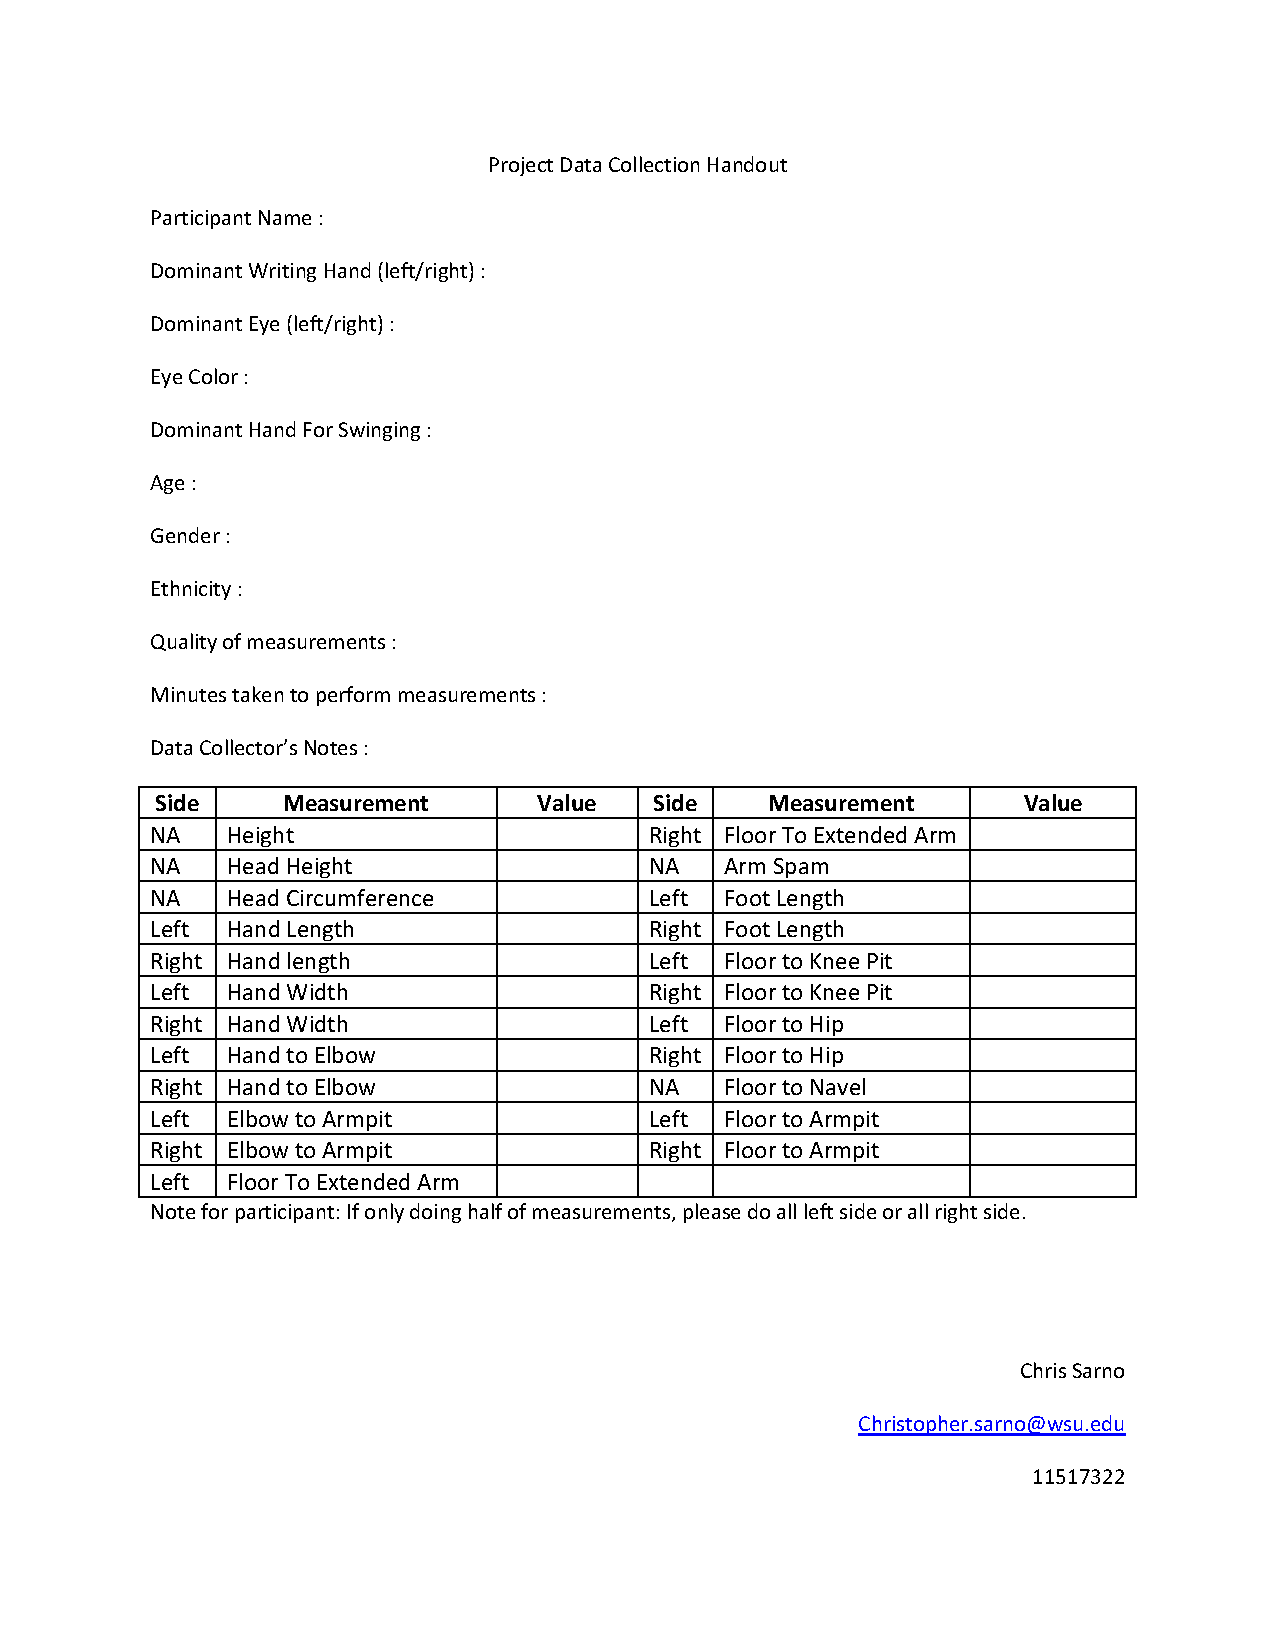
\includegraphics[trim = 0 0 0 0,clip,width=0.85\textwidth]{pdfs/Data-Handout.pdf} }
    \end{center}
    \label{fig:handout}
    \hrule
\end{figure}

\newpage

\subsection{Preparing the Report Workspace as a subsection}
\label{sec:appendix-setup}

\subsubsection{Preparing the Report Workspace as a subsubsection}
\label{sec:appendix-setup2}

\paragraph{Preparing the Report Workspace as a paragraph}
\label{sec:appendix-setup3}

\subparagraph{Preparing the Report Workspace as a subparagrah}
\label{sec:appendix-setup4}

Below is the necessary functions and libraries required to run the code
referenced in this document.

\begin{Shaded}
\begin{Highlighting}[]
\KeywordTok{library}\NormalTok{(devtools);       }\CommentTok{\# required for source\_url}

\NormalTok{path.humanVerseWSU =}\StringTok{ "https://raw.githubusercontent.com/MonteShaffer/humanVerseWSU/"}
\KeywordTok{source\_url}\NormalTok{( }\KeywordTok{paste0}\NormalTok{(path.humanVerseWSU,}\StringTok{"master/misc/functions{-}project{-}measure.R"}\NormalTok{) );}
\end{Highlighting}
\end{Shaded}

\begin{verbatim}
## Warning: package 'Hmisc' was built under R version 4.0.3
\end{verbatim}

Below is the code to load the data and prepare it for analysis.

\begin{Shaded}
\begin{Highlighting}[]
\NormalTok{path.project =}\StringTok{ "E:/Users/Mcshuggets/Documents/School/Math/Statistics/Stat 419 (Multivariate Statistics)/Project 1/Writeup material/"}\NormalTok{;}
\NormalTok{path.figures =}\StringTok{ "E:/Users/Mcshuggets/Documents/School/Math/Statistics/Stat 419 (Multivariate Statistics)/Project 1/Writeup material/figures/"}\NormalTok{;}

\NormalTok{path.to.secret =}\StringTok{ "E:/Users/Mcshuggets/Documents/School/Math/Statistics/Secret/"}\NormalTok{;}

\NormalTok{measure =}\StringTok{ }\NormalTok{utils}\OperatorTok{::}\KeywordTok{read.csv}\NormalTok{(}\KeywordTok{paste0}\NormalTok{(path.to.secret,}\StringTok{"measure{-}students.txt"}\NormalTok{), }\DataTypeTok{header=}\OtherTok{TRUE}\NormalTok{, }\DataTypeTok{quote=}\StringTok{""}\NormalTok{, }\DataTypeTok{sep=}\StringTok{"|"}\NormalTok{);}

\CommentTok{\#path.github = "https://raw.githubusercontent.com/this{-}IS{-}YOUR{-}PATH{-}TO{-}GITHUB/";}
\CommentTok{\#source\_url( paste0(path.github,"master/functions/functions{-}project{-}measure.R") );}

\CommentTok{\# this is your function}
\CommentTok{\# put in the same "units"}
\CommentTok{\# merge left/right}
\CommentTok{\# build proportion data}
\CommentTok{\# and so on ... }
\NormalTok{prepareMeasureData\textless{}{-}}\StringTok{ }\ControlFlowTok{function}\NormalTok{(file)}
\NormalTok{\{}
\NormalTok{  df \textless{}{-}}\StringTok{ }\KeywordTok{subset}\NormalTok{(file, }\DataTypeTok{select=}\KeywordTok{c}\NormalTok{(}\StringTok{"age"}\NormalTok{, }\StringTok{"height"}\NormalTok{,}\StringTok{"floor.hip"}\NormalTok{ ))}
\NormalTok{  df \textless{}{-}}\StringTok{ }\KeywordTok{na.omit}\NormalTok{(df)}
  \KeywordTok{return}\NormalTok{(df)}
\NormalTok{\}}
\NormalTok{measure.df =}\StringTok{ }\KeywordTok{prepareMeasureData}\NormalTok{(measure);}
\NormalTok{measure.df}\OperatorTok{$}\NormalTok{hip.head =}\StringTok{ }\NormalTok{measure.df}\OperatorTok{$}\NormalTok{height}\OperatorTok{{-}}\NormalTok{measure.df}\OperatorTok{$}\NormalTok{floor.hip}
\NormalTok{path.tables =}\StringTok{ }\KeywordTok{paste0}\NormalTok{(path.project,}\StringTok{"tables/"}\NormalTok{);}
  \KeywordTok{createDirRecursive}\NormalTok{(path.tables);}
\NormalTok{file.correlation =}\StringTok{ }\KeywordTok{paste0}\NormalTok{(path.tables,}\StringTok{"age{-}height{-}table.tex"}\NormalTok{);}

\NormalTok{measure.mrtx \textless{}{-}}\StringTok{ }\KeywordTok{as.matrix}\NormalTok{(measure.df)}
\KeywordTok{buildLatexCorrelationTable}\NormalTok{(measure.mrtx,}
  \DataTypeTok{rotateTable =} \OtherTok{FALSE}\NormalTok{,}
  \DataTypeTok{width.table =} \FloatTok{0.75}\NormalTok{,}
  \DataTypeTok{myFile =}\NormalTok{ file.correlation,}
  \DataTypeTok{myNames =} \KeywordTok{c}\NormalTok{(}\StringTok{"age"}\NormalTok{, }\StringTok{"height"}\NormalTok{, }\StringTok{"floor.hip"}\NormalTok{) );}
\end{Highlighting}
\end{Shaded}

Below is the code to generate the summary statistics and save them as a
table that you see in Section \ref{sec:data-sample}.

\begin{Shaded}
\begin{Highlighting}[]
\KeywordTok{summary}\NormalTok{(measure.df)}
\end{Highlighting}
\end{Shaded}

\begin{verbatim}
##       age            height        floor.hip        hip.head    
##  Min.   : 3.00   Min.   :36.61   Min.   :13.78   Min.   :17.13  
##  1st Qu.:22.00   1st Qu.:63.00   1st Qu.:35.98   1st Qu.:25.98  
##  Median :27.00   Median :66.50   Median :37.80   Median :28.66  
##  Mean   :34.89   Mean   :66.07   Mean   :37.51   Mean   :28.55  
##  3rd Qu.:52.00   3rd Qu.:70.00   3rd Qu.:39.76   3rd Qu.:30.51  
##  Max.   :94.00   Max.   :75.00   Max.   :44.49   Max.   :53.94
\end{verbatim}

\begin{Shaded}
\begin{Highlighting}[]
\KeywordTok{sink}\NormalTok{(}\StringTok{"summary.txt"}\NormalTok{)}
\KeywordTok{print}\NormalTok{(}\KeywordTok{summary}\NormalTok{(measure.df))}
\end{Highlighting}
\end{Shaded}

\begin{verbatim}
##       age            height        floor.hip        hip.head    
##  Min.   : 3.00   Min.   :36.61   Min.   :13.78   Min.   :17.13  
##  1st Qu.:22.00   1st Qu.:63.00   1st Qu.:35.98   1st Qu.:25.98  
##  Median :27.00   Median :66.50   Median :37.80   Median :28.66  
##  Mean   :34.89   Mean   :66.07   Mean   :37.51   Mean   :28.55  
##  3rd Qu.:52.00   3rd Qu.:70.00   3rd Qu.:39.76   3rd Qu.:30.51  
##  Max.   :94.00   Max.   :75.00   Max.   :44.49   Max.   :53.94
\end{verbatim}

\begin{Shaded}
\begin{Highlighting}[]
\KeywordTok{sink}\NormalTok{()}
\end{Highlighting}
\end{Shaded}

Below is the code to generate the graphs and correlation coefficients
referenced in Section \ref{sec:data-summary} and Section
\ref{sec:findings}.

\begin{Shaded}
\begin{Highlighting}[]
\CommentTok{\# Building the age vs height graph}
\KeywordTok{pdf}\NormalTok{(}\DataTypeTok{file=}\KeywordTok{paste0}\NormalTok{(path.figures, }\StringTok{"height{-}graph.pdf"}\NormalTok{))}
\KeywordTok{plot}\NormalTok{(measure.df}\OperatorTok{$}\NormalTok{age, measure.df}\OperatorTok{$}\NormalTok{height,}
     \DataTypeTok{pch =} \DecValTok{16}\NormalTok{, }\DataTypeTok{cex =} \FloatTok{0.7}\NormalTok{,}
     \DataTypeTok{main=}\StringTok{"Age vs Raw Height"}\NormalTok{,}
     \DataTypeTok{xlab=}\StringTok{"Age"}\NormalTok{,}
     \DataTypeTok{ylab=}\StringTok{"Height"}\NormalTok{,}
     \DataTypeTok{type=}\StringTok{"h"}\NormalTok{)}
\KeywordTok{abline}\NormalTok{(}\KeywordTok{lm}\NormalTok{(measure.df}\OperatorTok{$}\NormalTok{height}\OperatorTok{\textasciitilde{}}\NormalTok{measure.df}\OperatorTok{$}\NormalTok{age), }\DataTypeTok{col=}\StringTok{"red"}\NormalTok{)}
\KeywordTok{dev.off}\NormalTok{()}
\end{Highlighting}
\end{Shaded}

\begin{verbatim}
## pdf 
##   2
\end{verbatim}

\begin{Shaded}
\begin{Highlighting}[]
\KeywordTok{lm}\NormalTok{(measure.df}\OperatorTok{$}\NormalTok{height}\OperatorTok{\textasciitilde{}}\NormalTok{measure.df}\OperatorTok{$}\NormalTok{age)}
\end{Highlighting}
\end{Shaded}

\begin{verbatim}
## 
## Call:
## lm(formula = measure.df$height ~ measure.df$age)
## 
## Coefficients:
##    (Intercept)  measure.df$age  
##       65.41827         0.01858
\end{verbatim}

\begin{Shaded}
\begin{Highlighting}[]
\KeywordTok{cor}\NormalTok{(measure.df}\OperatorTok{$}\NormalTok{height, measure.df}\OperatorTok{$}\NormalTok{age)}
\end{Highlighting}
\end{Shaded}

\begin{verbatim}
## [1] 0.06154268
\end{verbatim}

\begin{Shaded}
\begin{Highlighting}[]
\CommentTok{\# Building the age vs hip to floor graph}
\KeywordTok{pdf}\NormalTok{(}\DataTypeTok{file=}\KeywordTok{paste0}\NormalTok{(path.figures, }\StringTok{"hip{-}floor{-}graph.pdf"}\NormalTok{))}
\KeywordTok{plot}\NormalTok{(measure.df}\OperatorTok{$}\NormalTok{age, measure.df}\OperatorTok{$}\NormalTok{floor.hip,}
     \DataTypeTok{pch =} \DecValTok{16}\NormalTok{, }\DataTypeTok{cex =} \FloatTok{0.7}\NormalTok{,}
     \DataTypeTok{main=}\StringTok{"Age vs Lower Half"}\NormalTok{,}
     \DataTypeTok{xlab=}\StringTok{"Age"}\NormalTok{,}
     \DataTypeTok{ylab=}\StringTok{"Length"}\NormalTok{,}
     \DataTypeTok{type=}\StringTok{"p"}\NormalTok{)}
\KeywordTok{abline}\NormalTok{(}\KeywordTok{lm}\NormalTok{(measure.df}\OperatorTok{$}\NormalTok{floor.hip}\OperatorTok{\textasciitilde{}}\NormalTok{measure.df}\OperatorTok{$}\NormalTok{age), }\DataTypeTok{col=}\StringTok{"red"}\NormalTok{)}
\KeywordTok{dev.off}\NormalTok{()}
\end{Highlighting}
\end{Shaded}

\begin{verbatim}
## pdf 
##   2
\end{verbatim}

\begin{Shaded}
\begin{Highlighting}[]
\KeywordTok{lm}\NormalTok{(measure.df}\OperatorTok{$}\NormalTok{floor.hip}\OperatorTok{\textasciitilde{}}\NormalTok{measure.df}\OperatorTok{$}\NormalTok{age)}
\end{Highlighting}
\end{Shaded}

\begin{verbatim}
## 
## Call:
## lm(formula = measure.df$floor.hip ~ measure.df$age)
## 
## Coefficients:
##    (Intercept)  measure.df$age  
##        36.5750          0.0269
\end{verbatim}

\begin{Shaded}
\begin{Highlighting}[]
\KeywordTok{cor}\NormalTok{(measure.df}\OperatorTok{$}\NormalTok{floor.hip, measure.df}\OperatorTok{$}\NormalTok{age)}
\end{Highlighting}
\end{Shaded}

\begin{verbatim}
## [1] 0.1281182
\end{verbatim}

\begin{Shaded}
\begin{Highlighting}[]
\CommentTok{\# Building the age vs hip to head graph}
\KeywordTok{pdf}\NormalTok{(}\DataTypeTok{file=}\KeywordTok{paste0}\NormalTok{(path.figures, }\StringTok{"hip{-}head{-}graph.pdf"}\NormalTok{))}
\KeywordTok{plot}\NormalTok{(measure.df}\OperatorTok{$}\NormalTok{age, measure.df}\OperatorTok{$}\NormalTok{hip.head,}
     \DataTypeTok{pch =} \DecValTok{16}\NormalTok{, }\DataTypeTok{cex =} \FloatTok{0.7}\NormalTok{,}
     \DataTypeTok{main=}\StringTok{"Age vs Upper Half"}\NormalTok{,}
     \DataTypeTok{xlab=}\StringTok{"Age"}\NormalTok{,}
     \DataTypeTok{ylab=}\StringTok{"Length"}\NormalTok{,}
     \DataTypeTok{type=}\StringTok{"p"}\NormalTok{)}
\KeywordTok{abline}\NormalTok{(}\KeywordTok{lm}\NormalTok{(measure.df}\OperatorTok{$}\NormalTok{hip.head}\OperatorTok{\textasciitilde{}}\NormalTok{measure.df}\OperatorTok{$}\NormalTok{age), }\DataTypeTok{col=}\StringTok{"red"}\NormalTok{)}
\KeywordTok{dev.off}\NormalTok{()}
\end{Highlighting}
\end{Shaded}

\begin{verbatim}
## pdf 
##   2
\end{verbatim}

\begin{Shaded}
\begin{Highlighting}[]
\KeywordTok{lm}\NormalTok{(measure.df}\OperatorTok{$}\NormalTok{hip.head}\OperatorTok{\textasciitilde{}}\NormalTok{measure.df}\OperatorTok{$}\NormalTok{age)}
\end{Highlighting}
\end{Shaded}

\begin{verbatim}
## 
## Call:
## lm(formula = measure.df$hip.head ~ measure.df$age)
## 
## Coefficients:
##    (Intercept)  measure.df$age  
##      28.843232       -0.008323
\end{verbatim}

\begin{Shaded}
\begin{Highlighting}[]
\KeywordTok{cor}\NormalTok{(measure.df}\OperatorTok{$}\NormalTok{hip.head, measure.df}\OperatorTok{$}\NormalTok{age)}
\end{Highlighting}
\end{Shaded}

\begin{verbatim}
## [1] -0.03887501
\end{verbatim}

\begin{Shaded}
\begin{Highlighting}[]
\CommentTok{\# Combining the lower half and upper half graphs}
\KeywordTok{pdf}\NormalTok{(}\DataTypeTok{file=}\KeywordTok{paste0}\NormalTok{(path.figures, }\StringTok{"combined{-}graph.pdf"}\NormalTok{))}
\KeywordTok{plot}\NormalTok{(measure.df}\OperatorTok{$}\NormalTok{age, measure.df}\OperatorTok{$}\NormalTok{hip.head,}
     \DataTypeTok{pch =} \DecValTok{16}\NormalTok{, }\DataTypeTok{cex =} \FloatTok{0.7}\NormalTok{,}
     \DataTypeTok{main=}\StringTok{"Lower vs Upper Half"}\NormalTok{,}
     \DataTypeTok{xlab=}\StringTok{"Age"}\NormalTok{,}
     \DataTypeTok{ylab=}\StringTok{"Length"}\NormalTok{,}
     \DataTypeTok{type=}\StringTok{"p"}\NormalTok{)}
\KeywordTok{abline}\NormalTok{(}\KeywordTok{lm}\NormalTok{(measure.df}\OperatorTok{$}\NormalTok{hip.head}\OperatorTok{\textasciitilde{}}\NormalTok{measure.df}\OperatorTok{$}\NormalTok{age), }\DataTypeTok{col=}\StringTok{"red"}\NormalTok{)}
\KeywordTok{abline}\NormalTok{(}\KeywordTok{lm}\NormalTok{(measure.df}\OperatorTok{$}\NormalTok{floor.hip}\OperatorTok{\textasciitilde{}}\NormalTok{measure.df}\OperatorTok{$}\NormalTok{age), }\DataTypeTok{col=}\StringTok{"blue"}\NormalTok{)}
\KeywordTok{text}\NormalTok{(}\DecValTok{50}\NormalTok{, }\DecValTok{40}\NormalTok{, }\StringTok{"Lower Half"}\NormalTok{)}
\KeywordTok{text}\NormalTok{(}\DecValTok{80}\NormalTok{, }\DecValTok{30}\NormalTok{, }\StringTok{"Upper Half"}\NormalTok{)}
\KeywordTok{dev.off}\NormalTok{()}
\end{Highlighting}
\end{Shaded}

\begin{verbatim}
## pdf 
##   2
\end{verbatim}

\begin{Shaded}
\begin{Highlighting}[]
\KeywordTok{lm}\NormalTok{(measure.df}\OperatorTok{$}\NormalTok{height}\OperatorTok{\textasciitilde{}}\NormalTok{measure.df}\OperatorTok{$}\NormalTok{age)}
\end{Highlighting}
\end{Shaded}

\begin{verbatim}
## 
## Call:
## lm(formula = measure.df$height ~ measure.df$age)
## 
## Coefficients:
##    (Intercept)  measure.df$age  
##       65.41827         0.01858
\end{verbatim}

\begin{Shaded}
\begin{Highlighting}[]
\KeywordTok{cor}\NormalTok{(measure.df}\OperatorTok{$}\NormalTok{age, measure.df}\OperatorTok{$}\NormalTok{height)}
\end{Highlighting}
\end{Shaded}

\begin{verbatim}
## [1] 0.06154268
\end{verbatim}




%% appendices go here!


\newpage
\theendnotes

%%%%%%%%%%%%%%%%%%%%%%%%%%%%%%%%%%%  biblio %%%%%%%%
\newpage
\begin{auxmulticols}{2}
\singlespacing 
\bibliography{./biblio/master.bib}

%%%%%%%%%%%%%%%%%%%%%%%%%%%%%%%%%%%  biblio %%%%%%%%
\end{auxmulticols}

\newpage
{
\hypersetup{linkcolor=black}
\setcounter{tocdepth}{3}
\tableofcontents
}



\end{document}